\section{The UTP Schema}
\label{sec:schema}
The \UTP{} schema %is used to model instances of educational timetabling problems.
%It
combines a schema to model timetabling entities and solutions, 
and a rule language.
% The \UTP{} schema enforces 
% a structured model to represent the entities of a problem instance, 
% and includes a rule language to express instance-specific constraints
% and a solution model to represent timetabling decisions.
The entity schema %enforces a structure
models the entities of a \UTP{} instance
- scheduling horizon, resources, and course elements including course sessions -,
their properties and relationships.
%The schema also includes a
The rule language is user-oriented
and serves to concisely express constraints
over any set of entities
on the different facets of a problem (e.g., session scheduling, capacity planning, resource allocation).
Rules are %user-oriented and 
formulated
using a catalog of timetabling constraint predicates
and a query language to select, filter and bind entities to sessions. 
 

A rule-based \UTP{} instance is 
converted
to a constraint-based instance
that is readily processable by solvers.
The conversion 
translates the entity schema as decision variables and core constraints, and then flattens rules as additional constraints.
A \UTP{} instance is thus cast as a hard constraint satisfaction problems.
Solving an instance involves scheduling sessions
and assigning them resources 
so that the core constraints and the rule constraints are satisfied.
The solution schema allows to represent
any timetabling solution computed for an instance,
be it incomplete or inconsistent.

This section introduces
the components of the schema.
The abstract syntax of the entity schema
is given in Table~\ref{table:entity-model},
its constraint-based modeling in
Table~\ref{table:core-variables} and
Table~\ref{table:core-constraints}
(Appendix~\ref{appendix:core-model}),
and the syntax of the rule language
and constraint predicates in
Table~\ref{tab:rule-language},
Table~\ref{tab:predicate_catalog} and
Table~\ref{tab:constraintformel}
(Appendix~\ref{appendix:constraintcatalog}).


\subsection{Entity Schema}
\label{sec:entity-schema}

% \subsubsection{Overview}
% \label{sec:entity-schema-overview}

The entity schema 
of a \UTP{} instance
combines
a hierarchy of course elements %namely, 
(i.e., courses, course parts, part classes and class sessions)
a scheduling horizon over which sessions are to be scheduled,
and 4 types of resources to which sessions must be allocated to
(i.e., rooms, teachers, students and student groups).
The schema encodes the nesting of course elements
and various properties and constraints 
concerning 
session scheduling,
resource availability, 
resource eligibility,
teaching service,
room capacity,
and student sectioning. %\todo{be more specific on sectioning? ie. out of scope}
% Session-related properties and constraints are either specified on individual sessions
% or inherited from course parts.
% All constraints are ultimately cast as domain, cardinality or assignment constraints on decision variables
% in the core model.

The scheduling horizon is a range
%$\SLOT$ 
of integers denoting \timepoints{}.
The \timepoints{} are the start and end times allowed for sessions
and any duration (i.e., session length, travel time and break time)
is measured as a number of \timepoints{}. 
The horizon is
defined using 3 instance fields: 
the number of weeks $\week$ dividing the horizon, 
the number of weekdays $\weekday$ making a week 
and the number of daily slots $\dailyslot$ making a 24-hour day.
The \timepoints{} correspond to all possible triplets combining a week, a weekday, and a daily slot. 
Note that daily slots may have any granularity (e.g., 1 minute, 2 hours)
and
%Besides, 
the scheduling horizon may be sparse
(e.g., if weeks $i$ and $i+1$ are not consecutive calendar weeks for some $1\leq i<\week$ 
or if weekdays are dropped, i.e., $\weekday<7$).
%If so, any duration exceeding a day or a week should be interpreted with care.

Course elements follow a hierarchical structure.
% nesting
% courses,
% %(set $\COURSE$),
% course parts,
% %(set $\PART$),
% part classes,
% %(set $\CLASS$),
% and class sessions.
% %(set $\SESSION$).
% %(\hyperref[feat:coursehierarchie]{``course hierarchy''}), 
Each course (e.g., Algorithms) consists of one or more parts (e.g., Lecture and Lab),
each part is taught to one or more classes (e.g., lecture classes A and B),
and all classes of a part have the same number of sessions (e.g., sessions 1 to 10 for each lecture class).
% The classes of a part share the same number of sessions.
%TODO \todo{@corentin: post-soumission, toutes les règles/assertions du schéma (eg. les classes d'1 part doivent avoir la même durée, inclusion entre required/possible, ordre en min/max) sont à compiler dans une section séparée de l'annexe.}
~The schema requires that all sessions in a class have the same duration
and be chronologically ranked,
i.e., session of rank $i+1$ in a class must start after session of rank $i-1$ ends in any solution.
These constraints are paramount to model course plans that rely on clear-cut sessions
(e.g., starting lab classes after 2 lecture sessions,
synchronizing the $5^{th}$ sessions of lab classes for a joint examination).
Besides, the schema allows to restrict the possible time slots for the sessions of a part
by setting allowed and forbidden ranges using the time format.
%Note that sessions are considered uninterruptible 
%and %, in particular, 
%may not overlap 2 days.
Note that 
sessions must start and end on the same day, and cannot be interruptible. % and cannot extend over two days.
%
The schema also specifies a set of possible resources for each session.
As for students, % and groups, 
a sectioning plan
%\footnote{Student sectioning consists in generating and matching student groups with classes consistently with course enrollments of students, class headcount thresholds and group sectioning policies (e.g., aggregating groups bottom-up from labs to lectures) or cross-course constraints (e.g., populating classes of different courses of a curriculum with identical groups).}
%\todo{comment-out footnote?}
is assumed and hard-coded together with group-to-class assignments.
Specifically, 
students are partitioned into groups,
and groups aggregated and assigned to classes
with no group being assigned to more than one class per course part.
The schema encodes group and class headcounts
as well as class headcount thresholds used for sectioning.%TODO \todo{@corentin: thresholds really needed in the models? Dicussion en réunion le size et le headcount en fonction du mode de fonctionnement }
~Other sectioning data and constraints %(e.g., course enrollments, group aggregation rules) 
are compiled away.
%but remains necessary for ...}
The implicit constraint to satisfy %to satisfy here %enforced on groups %enforced by the entity model 
is that a group must attend all the sessions of a class it is bound to.
%(\hyperref[feat:group]{``group''}). 

% As opposed to students, % and groups, 
Teacher-to-session assignments are not fixed
but subject to domain and cardinality constraints.
To meet practical needs, 
the schema allows multiple teachers per session
(e.g., joint supervision of a lab session) %, exam requiring several monitors)
and %as well as 
teacher-less sessions 
(e.g., unsupervised project work).
The number of teachers per session is specific to each course part
and is lower- and upper-bounded, possibly fixed.
Each part is also associated with 
a set of required teachers
and a superset of allowed teachers.
Hence two sessions of a class may be allocated different teachers and numbers of teachers.
A part also sets the fixed number of sessions a teacher is committed to.
% Again, this number may be fixed or bounded.
Overall, various demand and capacity requirements relating to teaching service 
can be addressed on course parts.
If needed, finer-grained rules may be imposed
(e.g., requiring the same staff for a class, naming a lecturer for a session).

Similarly, each part sets the required and possible rooms for its sessions and their number.
This caters for the case of multi-room sessions (e.g., for hybrid teaching)
and room-less sessions (e.g., field trips). %\todo{english SORTIE}
In addition, each part casts its sessions as room-exclusive or room-inclusive
which entails different allocation constraints.
A session is room-exclusive if none of the room(s) hosting it may simultaneously host another session.
Conversely, a room-inclusive session allows for its room(s) to be shared from start to finish.
While single-room sessions may be cast as exclusive or inclusive,
multi-room sessions may only be cast as exclusive.
That is, every session of a part whose room upper-bound is greater than 1 is considered exclusive. 
The rationale is that multi-room inclusive sessions have arguably little practical interest %in the timetabling domain.
and they also burden the computational model with decisions to make on the distribution of groups in shared rooms. 

All resources enforce capacity constraints w.r.t. their utilization.
%Since modalities differ from one environment to the next, 
Students, teachers and rooms are considered cumulative resources in this respect.
That is, they may attend, teach or host simultaneous sessions.
A cumulative model is paramount 
to satisfy flexible attendance requirements
(e.g., students attending tutoring sessions overlapping with compulsory courses)
and multi-class events 
(e.g., an amphitheater hosting %simultaneous exams or 
a joint conference for different classes).
Again, rules may be used to impose disjunctive resources 
or to ban session overlapping.
%
No limit is set on the number of parallel sessions teachers and students may attend.
Session hosting however is subject to capacity constraints
and the schema encodes the capacity of each room,
allowing for infinite capacity to handle virtual rooms. %\todo{@corentin: is the virtual room case covered in the models?} marc: oui
As discussed above, 
at any point in time, 
an allocated room will
either 
co-host a multi-room (exclusive) session
or host one or more single-room sessions (one only if a session is exclusive).
The schema hence enforces two kinds of capacity constraints.
The single-room case involves checking
if the total headcount of the session(s) falls below the room capacity.
The multi-room case involves
ensuring the total capacity of the rooms envisaged for the session exceeds its headcount.
If so, 
%As discussed above, 
no restriction is imposed as to the distribution of students in rooms
and whether it preserves group structure or not.

Lastly, the schema provides users with the ability to define their own classes of entities,
mixing course elements and resources as needed
with no limit on classification
(e.g., a block of rooms, the lecturers of a faculty department).
This is achieved by labeling entities.
Labels, built-in entity types and ids
are the building blocks of the query language
to forge rules for any group of entities.



% Similarly to the {\ITC} language, 
% the {\UTP} language adopts a multi-scale schedule horizon (i.e., weeks, weekdays and daily slots), a mixed set of resources (i.e., students, student groups, rooms and lecturers), and a hierarchical course structure (i.e., course parts, part classes and class sessions). In our approach however, class sessions (a.k.a., class meetings) are considered as first-class objects that must be scheduled individually alongside resources. 
% The model supports single-resource sessions (e.g., single lecturer) as well as multi-resource sessions (e.g., hybrid teaching), and encodes core constraints relating to student sectioning, session scheduling and resource allocation. %which are cast using built-in properties and relations over entities (i.e., resources and course elements) and sessions. 
% All resources are assumed cumulative (i.e., rooms, lecturers and students may host, teach and attend overlapping sessions) but this policy may be overridden with disjunctive scheduling rules.
% The rules language effectively allows to enforce additional constraints on selected sets of sessions and entities (i.e., resources and course elements).
% Rules are expressed using a catalog of timetabling predicates and a comprehension syntax to group, filter and bind sessions and entities. 
% Specifically, each rule denotes a conjunction of \UTP{} constraints sharing the same predicate (e.g., periodicity of all lecture classes of a course) and constraints are technically generated through a rule flattening process. %on selected classes of entities and sessions 

% %Specifically, the sessions of a course part are cast as single-resource (e.g., face-to-face lectures) or multi-resource sessions (e.g., hybrid sessions) by quantifying the needed resources. 
% %Lecturers and rooms are distributed over course parts while students are distributed over courses based on registrations which determines the resources allowed for each session.
% %%The resources allowed for a session follow from the distribution of student registrations over courses and that of lecturers and rooms over course parts. 
% %The volume of sessions per student depends on individual course registrations as class attendance is compulsory; it is configurable per lecturer in each course part but is unconstrained for rooms. 
% %%The volumes of sessions are configurable per teacher in each part (i.e., sessions quota) but pre-determined for students (i.e., class attendance is mandatory) and unconstrained for rooms. 
% %No limits apply on simultaneous resource usage but for rooms whose hosting capacity must match class size. Any resource may hence be allocated to joint or overlapping sessions  (e.g., lecture and optional tutoring for students) except for rooms hosting multi-room sessions. In any case, rules may be enforced as needed to prevent sessions from overlapping or to make resources fully disjunctive. As for session scheduling, start time grids are configurable in each course part and the model simply requires full session sequencing in each class. Lastly, the model sections students into classes and supports subgroup inclusion constraints between classes. Note that student groups are considered a by-product of student sectioning and as such may only be listed in the solution component. 

% %The rules language allows to state additional constraints using a catalog of timetabling predicates. A rule is tied to a predicate and models a conjunction of constraints on selected classes of entities and sessions (e.g., disjunctive scheduling rule for lecturers, temporal constraints on the courses of a curriculum). Each constraint applies to one or more pairs, called e-maps, and may involve parameters based on the predicate signature. An e-map either associates a resource with a subset of its compatible sessions or a course element with a subset of its constitutive sessions. In the first case, the e-map is interpreted as a set of conditional entity-to-session assignments while it is unconditional if it models a course element. Specifically, a constraint is only evaluated on the sessions for which its e-map argument(s) and the considered solution propose the same entity. Each predicate may be applied equally well to any type of e-map and be used to constrain resources (e.g., lecturer unavailability), course elements (e.g., class periodicity) or individual sessions (e.g., session parallelization). %Note that constraints on e-maps modeling sessions of course elements are de facto unconditional. 
% %Formally, a rule is defined by a universally quantified formula wherein quantifiers restrict the domains of the e-map variables. A language of selectors is provided to build and filter domains of e-maps based on session ranks, entity identifiers, entity types, or any user-defined class of elements (e.g., team of lecturers, block of rooms). A rule hence denotes the conjunction of constraints obtained by instantiating the predicate over the cross-product of the domains of the e-map variables. 

% \todo{david toolchain figure? uncomment}
% % \begin{figure}
% %     \centering
% %     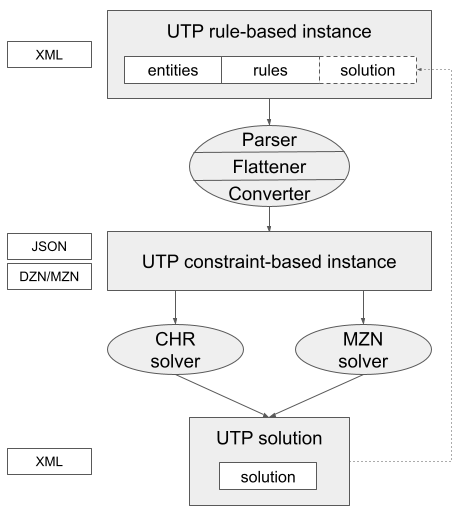
\includegraphics[scale=0.4]{img/utp_toolchain.png}
% %     \caption{The \UTP{} toolchain.}
% %     \label{fig:toolchain}
% % \end{figure}

% Note that all constraints are handled as hard constraints and each {\UTP} instance is reduced to a hard constraint satisfaction problem ({\CSP}).
% The ability to model preferences and multi-criteria objectives by the means of soft constraints is paramount in course timetabling and will be the subject of future extensions. 
% Likewise, the catalog of {\UTP} predicates still lacks important constraints (e.g., gap, distribution and pattern constraints - see e.g. \cite{2017_aizam_AIPCP,2021_chen_IEEEA}) which will be gradually added in future versions.

% \subsubsection{Data Model}
% \label{sec:entity-schema-model}
Table~\ref{table:entity-model} provides a formal specification of the schema elements.
Resources and course elements, except sessions, are referred to as \textit{entities}.
Entities are typed,
the set of sessions is cast as distinct type, 
and each type is modeled as a finite set.
% % :
% % the set of courses ${\COURSE}$, 
% % course parts ${\PART}$, 
% % classes ${\CLASS}$, 
% % teachers ${\TEACHER}$,
% % rooms ${\ROOM}$,
% % students ${\STUDENT}$, 
% % student groups ${\GROUP}$, 
% % and the domain of courses %${\COURSES}$ 
% % ${\COURSES}=\myset{\COURSE}$. 
% % ${\TYPE}$
% % (
% $
% {\TYPE}
% =
% \myset{
% {\COURSES}, 
% {\COURSE},
% {\PART},
% {\CLASS},
% {\ROOM},
% {\TEACHER},
% {\STUDENT},
% {\GROUP}
% }
% $
% % )
% denotes the set of entity types, 
% % ${\ENTITY}$
% ${\ENTITY}=\setunion{X}{\TYPE}{X}$
%  the set of entities,
% and ${\SESSION}$ the set of sessions.
The course element hierarchy
defines 1-to-many \textit{composition relations} over the pair of types
$(X,Y)$ corresponding to parent and child types
in the course element hierarchy. 
Each relation is modeled by a function ${\maptype{X}{Y}}:X\rightarrow2^{Y}$
mapping each object $i$ of type $X$
to the set ${\map{X}{Y}{i}}$ of its constitutive objects of type $Y$.
% For notational convenience, the table also represents the inverse ${\maptype{Y}{X}}:Y\rightarrow2^{X}$ of each function ${\maptype{X}{Y}}$.
% ($j\in\map{X}{Y}{i}\leftrightarrow i\in\map{Y}{X}{j}$)
For instance, 
${\maptype{\PART}{\CLASS}}$ 
models the classes of each part.
% and ${\maptype{\CLASS}{\PART}}$ 
% the (singleton) part of each class.
Each \textit{compatibility relation}
defining the allowed or assigned resources of a course element object
for a given resource type and course element type
defines a many-to-many relation
which we model the same way.
%by 2 inverse functions.
For instance, 
${\maptype{\PART}{\ROOM}}$
models the allowed rooms per part
and ${\maptype{\CLASS}{\GROUP}}$
the set of groups assigned to classes.

For notational convenience, 
the table also defines 
the maps resulting from 
the symmetric and transitive closure of the binary relation %(digraph)
merging the composition and compatibility maps.
This includes
the maps
computed over the course tree.
% \footnote{
% $\forall X,Y,Z \in {\TYPE}\cup\myset{\SESSION}:
% X\preceq^{*} Y\preceq^{*} Z 
% \Rightarrow 
% (\forall i \in X:
% \map{X}{Z}{i}=\setpartition{j}{\map{X}{Y}{i}}{\map{Y}{Z}{j}}
% $
% }
For instance, 
%function 
${\maptype{\CLASS}{\PART}}$ 
models the (singleton) part of each class,
and ${\maptype{\COURSE}{\SESSION}}$ 
the sessions of a course.
%resulting from the recursive set-union of the sessions of its parts' classes.
This also includes the 
inverse compatibility constraints
and those inherited along the course tree.
For instance, ${\maptype{\SESSION}{\ROOM}}$ models the rooms allowed for a session
which results from the composition of ${\maptype{\SESSION}{\CLASS}}$, ${\maptype{\CLASS}{\PART}}$ and ${\maptype{\PART}{\ROOM}}$.
% - 
% $
% j\in{\map{\SESSION}{\ROOM}{i}}
% \leftrightarrow 
% j\in{\map{\PART}{\ROOM}{k}}
% \wedge
% i\in{\map{\PART}{\SESSION}{k}}
% $
% )
Lastly, the table defines the constants (e.g., number of weeks),
scalar properties
(e.g., room capacity),
and remaining relations and sets (e.g. required resources, labels).
% and remaining relations (required resources) 
% and sets (labels, exclusive/inclusive sessions).

% $
% {\prec}
% =
% \myset{
% ({\COURSES},{\COURSE}),
% ({\COURSE},{\PART}),
% ({\PART},{\CLASS}),
% ({\CLASS},{\SESSION}),
% ({\TEACHER},{\PART}),
% ({\ROOM},{\PART}),
% ({\STUDENT},{\GROUP}),
% ({\GROUP},{\COURSE})
% }
% $
% denotes the relation over 
% ${\TYPE}\cup\myset{\SESSION}$ 
% that models the course hierarchy
% and the distribution of resource types over course components.

% ${\prec^{*}}$
% %${\preceq^{*}}$
% denotes the transitive %and reflexive 
% closure of
% ${\prec}$ 
% over
% ${\TYPE}\cup\myset{\SESSION}$
% and
% ${\maptype{X}{Y}}:X\rightarrow2^{Y}$
% denotes the function mapping each element of $X$ to its set of compatible elements in $Y$
% for each pair %$(X,Y)$ such that 
% %$X{\preceq^{*}}Y$.
% $X{\prec^{*}}Y$.
% For instance, 
% ${\maptype{\ROOM}{\PART}}$ 
% represents the distribution of rooms over course parts, 
% ${\maptype{\PART}{\CLASS}}$ 
% the decomposition of course parts into classes,
% ${\maptype{\CLASS}{\SESSION}}$ 
% the decomposition of classes into sessions,
% and ${\maptype{\ROOM}{\SESSION}}$ 
% the inferred distribution of rooms over sessions.
% The functions corresponding to the pairs of $\prec$
% are directly encoded in the entity model
% and the remaining functions are defined inductively using recursive aggregation. 

% We shall denote by ${\map{X}{Y}{i}}$ the image of entity $i$ of type $X$ over $2^Y$ %, i.e., the set of elements of type $Y$ compatible with $i$. 
% and by ${\maptype{Y}{X}}$ the inverse of ${\maptype{X}{Y}}$.

% Equation (\ref{model:hierarchy}) below models the hierarchical decomposition of course elements\footnote{$\disjunion$ denotes the disjoint union operation, i.e. set union over pairwise disjoint sets.},
% Equation (\ref{model:transitivity}) is the closure rule over 
% %$\preceq^{*}$. 
% $\prec^{*}$,
% %Note that each map $\maptype{\SESSION}{X}$ is the inverse of map $\maptype{X}{\SESSION}$.
% and Equation (\ref{model:inverse}) models inverse maps.

% \begin{align}
% %
% \forall (X,Y) \in 
% \myset{
% ({\COURSES},{\COURSE}),
% ({\COURSE},{\PART}),
% ({\PART},{\CLASS}),
% ({\CLASS},{\SESSION})
% }:
% Y=
% \setpartition{i}{X}{\map{X}{Y}{i}} 
% \label{model:hierarchy}
% \\
% %
% \forall X,Y,Z \in {\TYPE}\cup\myset{\SESSION}:
% X\preceq^{*} Y\preceq^{*} Z 
% \Rightarrow 
% (\forall i \in X:
% \map{X}{Z}{i}=\setpartition{j}{\map{X}{Y}{i}}{\map{Y}{Z}{j}}
% \label{model:transitivity})
% \\
% %
% \forall X,Y \in {\TYPE}:
% X\preceq^{*} Y 
% \Rightarrow 
% (\forall i \in X, j \in Y:
% j \in \map{X}{Y}{i} \Leftrightarrow i \in \map{Y}{X}{j}
% )
% \label{model:inverse}
% %\\
% %%
% %\forall X \in {\TYPE}\cup\myset{\SESSION},
% %i \in X:
% %\domarg{X}{X}{i} = \myset{i} \label{model:selfmap}
% %%
% \end{align}


%\footnote{
% The following rules apply. $\SLOT=\myset{i.\WEEKDAY.\DAILYSLOT+j.\DAILYSLOT+k\ |\ 0\leq i<\WEEK,0\leq j<\WEEKDAY,1\leq k\leq\DAILYSLOT}$.
% For each class $k$ in part $p$,
% $\myset{\sessionrank{s}\ |\ s\in\map{\CLASS}{\SESSION}{k}}=\myset{1,\ldots,\mycard{\map{\CLASS}{\SESSION}{k}}}$, 
% %$\mycard{\classparents{k}}\leq1$ 
% and $\classparents{k}\not\subset\map{\PART}{\CLASS}{p}$.
% For each pair of sessions $s,s'$, 
% $(s,s')\in\sessionranked$ iff $\map{\SESSION}{\CLASS}{s}=\map{\SESSION}{\CLASS}{s'}$ and $\sessionrank{s'}=\sessionrank{s}+1$.
% For each course part $p$,
% %$p\in\multiroomparts$ iff $\multiroompart{p}$; 
% %and 
% $\partteachermultiplicity{p}.\mycard{\map{\PART}{\SESSION}{p}}=\sum\limits_{l\in\map{\PART}{\TEACHER}{p}}{\partteacherservice{l,p}}$.}
%
%We shall denote by
%${\RANK}$
%the range of session ranks,
%${\maptype{\RANK}{\SESSION}}:\RANK\rightarrow2{^\SESSION}$
%the rank-based partitioning of sessions,
%and
%${\LABEL}$
%the set of labels 
%(${\LABEL}\subseteq2^{{\ENTITY}}$)
%completed 
%with the whole set of entities %to mock label optionality
%($\ENTITY\in{\LABEL}$)
%and singleton entities %to support identity-based selection
%($\myset{\myset{e}\ |\ e\in{\ENTITY}}\subseteq{\LABEL}$).
%As discussed in section~\ref{sec:rules},
%labels are optional filters used in rules to select entities
%hence the formal inclusion of $\ENTITY$ in ${\LABEL}$ to mock label optionality.
%Likewise, entity identifiers are used as an alternative to labels
%hence the inclusion of singleton entities in ${\LABEL}$.


\begin{table}[!t]
\begin{center}
\rowcolors{1}{gray!25}{white}
%\begin{tabular}{|r>{\columncolor{gray!25}}l|}
%\begin{tabular}{|ll|}
\begin{tabular}{|l|l|}
%\begin{tabular}{ll}


\hline
$\week$                                 & number of weeks
dividing the scheduling horizon
%in $\SLOT$\\
\\%in $\SLOT$\\
$\weekday$                               & number of weekdays
making a week \\
$\dailyslot$                              &  number of daily slots
making a 24-hour day% in $\SLOT$
%DAILY SLOT M pour minute
\\
$\WEEK =\myset{1,\ldots\week}$
&  range of weeks 
\\
$\WEEKDAY =\myset{1,\ldots\weekday}$
&  range of weekdays 
\\
$\DAILYSLOT =\myset{1,\ldots\dailyslot}$
&  range of daily slots 
\\
$\SLOT=\myset{1,\ldots\week\times\weekday\times\dailyslot}$
%$\SLOT$                                  
&  range of \timepoints{} (schedule horizon)
%defining the scheduling horizon
\\\hline
$\COURSE$%\subseteq\ENTITY$
                                            &  courses
\\
$\PART$%\subseteq\ENTITY$
                                            &  course parts
\\
$\CLASS$%\subseteq\ENTITY$
                                            &  part classes
\\
$\ROOM$%\subseteq\ENTITY$
                                            &  rooms
\\
$\TEACHER$%\subseteq\ENTITY$
                                            &  teachers
\\
$\STUDENT$%\subseteq\ENTITY$
                                            &  students
\\
$\GROUP$%\subseteq{\ENTITY}$
                                            &  groups of students

% \\
% $\ENTITY$                                   & the entities
\\\hline
$\COURSES=\myset{\COURSE}$%\subseteq\ENTITY$
                                            &  course domain
\\
$\TYPE=\myset{\COURSES,\COURSE,\PART,\CLASS,\ROOM,\TEACHER,\STUDENT,\GROUP}
$                                           &  types of entities
\\
${\ENTITY}=\setunion{X}{\TYPE}{X}$          &  set of entities
\\
$\map{X}{Y}{i}\subseteq{Y}, X \in \myset{\COURSES,\COURSE,\PART,\CLASS}$
                                            &  set of entities of type $Y$ tied to entity $i$ of type $X$
\\
$\map{X}{Y}{i}\subseteq{Y}, X \in \myset{\ROOM,\TEACHER,\STUDENT,\GROUP}$
                                            &  set of entities of type $Y$ associated with entity $i$ of type $X$
\\
% \\\hline
${\LABEL}\subseteq2^{{\ENTITY}}$            &  labels
\\\hline
% $\SESSION$                                  & the class sessions
% \\
$ \SESSIONEX$% \subseteq \SESSION $
                                            &  exclusive class sessions 
\\
$ \SESSIONINC$% \subseteq \SESSION $
                                            &  inclusive class sessions 
\\
$\SESSION=\SESSIONEX\disjunion\SESSIONINC$  &  class sessions
\\
$\partallowedslots{s}\subseteq{\SLOT}$      &  start times allowed for session $s$
\\
$\map{\SESSION}{X}{s}\subseteq{X}$
                                            &  set of entities of type $X$ tied to session $s$
\\
$\map{X}{\SESSION}{i}\subseteq{\SESSION}$
                                            &  set of sessions tied to entity $i$ of type $X$
% \\
% %UP
% $\umap{X}{\SESSION}{i}\subseteq{\SESSION},\; X\in\{\ROOM, \TEACHER\}$
%                                             & the set of sessions allowed for, or tied to, entity $i$ of type $X$
\\
%DOWN
$\dmap{X}{\SESSION}{i}\subseteq{\SESSION}$
                                            &  set of sessions required by resource entity $i$ of type $X$
\\
%$\disjunctiverooms\subseteq{\ROOM}$         & the set of disjunctive rooms
%\\
\hline
$\multiroompartmin{p}\in{\NATURAL}$          &  min number of rooms usable by each session of part $p$
%whether course part $p$ is multi-room or not
\\
$\multiroompartmax{p}\in{\NATURAL}$          &  max number of rooms usable by each session of part $p$
% whether course part $p$ is multi-room or not
\\
%$\partteachermultiplicity{p}\in{\NATURAL}$  & the number of lecturers usable by each session of part $p$
%\\
$\partteachermultiplicitymin{p}\in{\NATURAL}$  &  min number of lecturers usable by each session of part $p$
\\
$\partteachermultiplicitymax{p}\in{\NATURAL}$  &  max number of lecturers usable by each session of part $p$
\\
$\headcount{g}\in{\NATURAL}$               &  headcount of group $g$
\\
$\classcapacity{k}\in{\NATURAL}$            &  headcount of class $k$
\\
%$\multiteacherparts\subseteq{\PART}$           & the multi-teacher parts
%\\
%$\partteacherservice{l,p}\in{\NATURAL}$     & the number of sessions %required by lecturer $l$ in part $p$
%\\
$\roomcapacity{r}\in{\NATURAL}$             &  capacity of room $r$
\\
$\sessionduration{s}\in{\SLOT}$             &  duration of session $s$
\\
$\sessionrank{s}\in{\NATURAL^*}$            &  rank of session $s$ in its class
\\
$\partteacherservice{t,p}\in{\NATURAL}$     &  number of sessions required by teacher $t$ in part $p$
%\\
%$\sessionranked\subseteq{\SESSION\times\SESSION}$ & the pairs of sessions with consecutive ranks in a class
%\\
%$\sessionranked\subseteq{\SESSION\times\SESSION}$ & the pairs of sessions with consecutive ranks in a class
%$\classparents{k}\subseteq{\CLASS}$          & the parent classes of class $k$ if any
%\\
%\\
%$\virtualroom{r}\in{\BOOLEAN}$              & whether room $r$ is virtual or not
%\\
%$\virtualrooms\subseteq{\ROOM}$             & the virtual rooms
\\\hline
%$\PARTREQUIREDROOM \subseteq \CLASS$          & the classes requiring at least one room
% \\
%$\multiroomparts\subseteq{\PART}$           & the multi-room parts
%\\
%$\mandatoryrooms{p}\subseteq{\ROOM}$        & the mandatory rooms of part $p$
%\\
%
%
%$\multiroompart{p}\in{\BOOLEAN}$            & whether course part $p$ is multi-room or not
%\\
%\\\hline
\end{tabular}
\caption{Core data model.}
\label{table:entity-model}
\end{center}
\end{table}
%TODO \todo{for future work: the type graph/relation and its closure should be re-included in the text, and defined in the table and the maps `d` in the table explicitly restricted to pairs of the closed relation}

% ------------------------------------------------------------
% ------------------------------------------------------------
\subsection{Solutions}
\label{sec:solution}

The solution schema is used to encode
any solution pre-computed for an instance.
%(e.g., the choice of rooms and start times for sessions).
Such a solution needs not be complete, nor consistent with the instance constraints.
An instance may hence be associated with any kind of input solution based on the
computational task,
e.g. no solution at all when generating a timetable from scratch, 
a resource allocation solution to extend into a complete timetable,
a seed solution to improve, 
or an inconsistent solution to repair.
Formally, the solution schema
supports the representation of
any decision made for a session
as to its start time,
% on time points ($\var{\SESSION}{\SLOT}{s}$),
its set of rooms
%($\var{\SESSION}{\ROOM}{s}$)
and its set of teachers.
%($\var{\SESSION}{\TEACHER}{s}$)
%for sessions.

% the 
% on time points ($\var{\SESSION}{\SLOT}{s}$),
% rooms ($\var{\SESSION}{\ROOM}{s}$)
% and lecturers ($\var{\SESSION}{\TEACHER}{s}$)
% for sessions.



%------------------------------------------------------------
%------------------------------------------------------------
\subsection{Predicates, Constraints and Rules}
\label{sec:schema-predicates-constraints-rules}

The \UTP{} schema comes with a rule language to formulate instance-specific constraints.
Rule constraints add to the built-in constraints of the schema
and all must be checked when evaluating a solution.
The rule language is designed to target groups of entities, or individual entities,
and constrain the scheduling of their sessions
from any standpoint
(e.g., an institutional rule imposing a time structure on curricula,
a disjunctive scheduling rule applied to student groups,
a rule modeling the service plan within a faculty department,
a rule for a lecturer's agenda).
%the unavailability of department staff).
% Each rule provides a compact representation
% of a conjunction of constraints on selected entities and sessions.
The schema comes with a catalog of timetabling predicates
to build rules and compile them into constraints.
It also includes a custom syntax to select
selected entities and sessions on which rules apply.
%to forge rules on selected entities and sessions.


% Both the constraint syntax and query language
All these components are designed around the concept of \textit{e-map}.
Formally, an e-map is a pair $(e_i,S_i)$ 
mapping an entity $e_i$ to a set $S_i$ of sessions.
The query language is used to forge queries that retrieve sets of e-maps.
Each query selects, filters and binds entities to sessions from instance data 
in order to extract one or more sets of e-maps.
% before assembling them into tuples.
Each rule is bound to a predicate and scoped by a query.
At flattening time, 
the query is performed to retrieve a fixed number of sets of e-maps.
The rule is then compiled into a conjunction of constraints
by computing the cross-product of the extracted sets %of e-maps
and applying the predicate to each tuple of e-maps in the cross-product.
Constraint e-maps act as guards when checking solutions
and they also narrow the scope of interpretation.
The rationale is to discard constraints that are irrelevant
(e.g., a teacher's constraint forbidding afternoon lectures while the solution only assigns him lab sessions)
and, more generally, to limit constraint checks to the proposed assignments
(e.g., checking the above lecturer's constraint on the actual lectures the solution assigns him).
% E-maps may be classified as course or resource e-maps based on their entity.

As mentioned above, 
each %\UTP{} 
constraint applies a predicate to a tuple of e-maps.
\UTP{} predicates %accept one or more e-map variable arguments.
%They 
either accept a fixed number of %have a fixed arity (the number of 
e-maps % variables % arguments)
or are variadic.
Their semantics may be indifferent to the ordering of their arguments or not,
and some accept parameters.
Besides, each predicate may be used indistinctly
with course e-maps or resource e-maps (i.e., e-maps pairing course elements or resources),
and any n-ary constraint may freely mix the two types
(e.g., a constraint booking rooms for sessions involving different classes).
Let ${\EMAP}=\ENTITY\times{2^{\SESSION}}$ denote the domain of e-maps,
% defined by
% and defined by:
% \begin{equation*}
% {\EMAP}=
% \setunion{X}{\TYPE}
% \myset{(e,S')\ |\ e\in X,
% %\emptyset\subset 
% S'\subseteq\map{X}{\SESSION}{e}}
% \end{equation*}
the general form of a %n-ary %{\UTP} 
constraint is
% \begin{equation*}
% \begin{align}
$c((e_1,S_1),\ldots,(e_n,S_n),p_1,\ldots,p_m)$ %\label{rule:constraint}
% \end{align}
% \end{equation*}
where 
$c$ is a predicate of arity $n$,
$(e_1,S_1),\ldots,(e_n,S_n)$ are e-maps ($(e_i,S_i)\in{\EMAP}$ for $i=1\ldots n$) 
and 
$p_1,\ldots,p_m$ are values for the parameters of $c$ ($m\geq0$).

The semantics of constraints relies on a join operation between constraint e-maps and solutions.
% The pairing of entities and sessions to form e-maps
% is subject to typing rules imposed by the instance schema.
% Specifically, a course element (class, part, course or course domain)
% may only be paired with some of its constitutive sessions,
% whereas a resource 
% may only be paired with some of its allowed sessions 
% (or fixed sessions in the case of students and groups).
% %consistently with the instance schema data.
% E-maps may hence be classified as course or resource e-maps.
% We associate an e-map variable to each entity of the instance
% to denote the set of sessions it is assigned in a solution.
% Course e-map variables are actually constants 
% since each one represents the fixed set of constitutive sessions of a course element.
% Resource e-map variables however do vary since sessions have to be chosen for each resource.
Note first that any solution may be cast as a tuple of e-maps 
by converting the session-to-resource assignments into resource e-maps
and re-encoding the fixed maps binding course elements to their sessions.
We say an e-map is \textit{null} if it pairs an entity with an empty set of sessions,
and, by extension, a tuple of e-maps is null if it includes a null e-map.
Given a solution and an e-map for some entity,
we call \textit{joint e-map} the pairing of the entity with the set of sessions
on which the solution and the e-map agree,
i.e., the set-intersection of the sessions of the e-map and those assigned/bound to the entity in the solution encoding.
We say a solution is \textit{inconsistent} with an e-map if their joint e-map is null.
The join operation extends to tuples by performing the operation component-wise
%By extension, %a tuple of e-maps may be joined with a solution by joining individual e-maps
and a solution is said to be inconsistent with a tuple of e-maps 
if its is inconsistent with at least one e-map in the tuple.

%As for satisfiability, 
% t
The evaluation of a solution against a constraint
%(to decide whether it is satisfied or not)
% depends on the consistency of its e-map tuple with the solution.
is conditioned by the tuple of e-maps joining those of the solution and the constraint.
If the joint tuple is null, 
the constraint is considered satisfied
(i.e., it is deemed irrelevant and discarded).
% that is, it is deemed irrelevant and hence discarded
% (e.g., a constraint forbidding afternoon lectures while the solution does not include any).
Otherwise, the predicate is evaluated on the joint e-map
and the result depends on its built-in semantics.
% \footnote{Formally, 
% a constraint 
% $c((e_1,S_1),\ldots,(e_n,S_n),p_1,\ldots,p_m)$
% is satisfied by a solution
% verifying
% $\var{X}{\SESSION}{e_i}=S'_i$ ($i=1\ldots n$)
% iff
% there exists $i\in\myset{1,\ldots,n}$ s.t. $S_i\cap S'_i=\emptyset$
% or else
% $c((e_1,S_1\cap S'_1),\ldots,(e_n,S_n\cap S'_n),p_1,\ldots,p_m))$
% holds true.}
Specifically, the predicate is assessed on
the tuple of sets obtained by substituting each set of sessions
in the joint e-map
either by the set of their assigned start times,
or the set of their assigned resources of a given type (rooms, etc).
Which type (time or resource type) to pick per e-map is fixed and predicate-specific
(e.g., a temporal predicate will substitute any e-map argument by start times).
Note that entities play no role in the evaluation %of e-map tuples
once the join and substitution operations are over:
each predicate is ultimately evaluated on sets made of start times or sets of resources.
Note also that join operations leave course e-maps unchanged unlike resource e-maps.
This means constraints applying exclusively to course e-maps are de facto unconditional. 

% course e-maps 
% E-maps bound to resources are interpreted as conditional session-to-resource assignments
% when checking constraints
% whereas e-maps defined on course elements are unconditional assignments since they model constitutive sessions.
% It follows that 
% a constraint is evaluated on every session that is mapped to a course element by one of its e-map arguments.
% Constraints that apply exclusively to course elements are therefore unconditional. 
% Note also that the use of e-maps that model the whole set of sessions compatible with an entity 
% will necessarily constrain any session that may be assigned to this entity.

The \UTP{} catalog provides predicates to cover the various dimensions of time--tabling problems.
Some only address scheduling (i.e., start times),
others room allocation, and so on.
Table~\ref{tab:predicate_catalog} and Table~\ref{tab:constraintformel} given in Appendix~\ref{appendix:constraintcatalog} describe the predicates of the catalog and provide their semantics.
%of the language
%and indicates which are variadic or parametric.
Syntactically, each rule binds a predicate to a query
and denotes the conjunction of constraints obtained 
by applying the predicate to
each tuple of e-maps extracted by the query.
% Note that a query actually retrieves one or more sets of e-maps
% and does not explicitly compute their cross product.
% Formally, a rule is a universally quantified formula 
% wherein each quantifier restricts the domain of one of the e-map variables. 
%A language of selectors is provided to build and filter domains of e-maps based on session ranks, entity identifiers, entity types, or any user-defined class of elements (e.g., team of lecturers, block of rooms). A rule hence denotes the conjunction of constraints obtained by instantiating the predicate over the cross-product of the domains of the e-map variables. 
% Let 
% ${\SELECTOR}$
% denote the language of e-map domain selectors,
% %(${\SELECTOR}\subseteq({\TYPE}\times{\LABEL}\times{2^{\RANK}})^{n}$).
A %{\UTP} 
rule has the form %is a tuple 
% \begin{align}
$c\langle{\SELECTOR},p_1,\ldots,p_m\rangle$
% $r_c(F_1,\ldots,F_m,p_1,\ldots,p_n)$
% \end{align}
and is interpreted by %The semantics of a rule $(c,D_1,\ldots,D_m,p_1,\ldots,p_n)$ is 
the %quantified 
formula
\begin{equation*}
% \begin{flalign}
\forall (e_1,S_1)\in\denote{\SELECTOR_1},\ldots,(e_n,S_n)\in\denote{\SELECTOR_{n}}: c((e_1,S_1),\ldots,(e_n,S_n),p_1,\ldots,p_m)
% \forall (e_1,S_1)\in\denote{F_1},\ldots,(e_m,S_m)\in\denote{F_{m}}: c((e_1,S_1),\ldots,(e_m,S_m),p_1,\ldots,p_n)
%&\label{rule:rule}
% \end{flalign}
\end{equation*}
where 
$c$ is a predicate of arity $n$ accepting $m$ parameters ($m\geq0$),
$\SELECTOR$ is a query sized to extract $n$ sets of e-maps,
$\denote{\SELECTOR_i}$
denotes the $i$-th set of e-maps extracted with $\SELECTOR$
 (%$F_i\in{\SELECTOR}$, 
$i=1\ldots n$),
% $
% F_i\in{\SELECTOR}
% $,
and
$p_1,\ldots p_m$ are values for the parameters of $c$.




% E-maps bound to resources are interpreted as conditional session-to-resource assignments
% when checking constraints
% whereas e-maps defined on course elements are unconditional assignments since they model constitutive sessions.
% It follows that 
% a constraint is evaluated on every session that is mapped to a course element by one of its e-map arguments.
% Constraints that apply exclusively to course elements are therefore unconditional. 

% Note also that the use of e-maps that model the whole set of sessions compatible with an entity 
% will necessarily constrain any session that may be assigned to this entity.

% In the first case, the e-map is interpreted as a set of conditional entity-to-session assignments while it is unconditional if it models a course element. 
% Specifically, a constraint is only evaluated on the sessions for which its e-map argument(s) and the considered solution propose the same entity. 
% Each predicate may be applied equally well to any type of e-map and be used to constrain resources (e.g., lecturer unavailability), course elements (e.g., class periodicity) or individual sessions (e.g., session parallelization). 
% Note that constraints on e-maps modeling sessions of course elements are de facto unconditional. 

% A rule is tied to a predicate and models a conjunction of constraints on selected classes of entities and sessions (e.g., disjunctive scheduling rule for lecturers, time constraints on the courses of a curriculum).
%For instance, unconditional start time restrictions using predicates such as {\SAMEDAILYSLOT} or {\FORBIDDENPERIOD}  may be enforced on any set of sessions bound to a course, a part, a class or more generally to the course domain. Conversely, start time restrictions on a set of sessions bound to a resource will only be enforced on those which are eventually assigned to the resource.
%Predicates serve to constrain the possible sessions of resources (e.g., unavailabilities of a teacher) or the constitutive sessions of course elements (e.g., periodicity of a class). 
%e-maps may then be adjusted to constrain candidate sessions of resources (e.g., teacher unavailability), constitutive sessions of course elements (e.g., class periodicity), or individual sessions (e.g., session sequencing and parallelization).

% All {\UTP} constraints apply to pairs, called e-maps,
% which associate an entity with a set of sessions.
% % Specifically, 
% % an e-map
% % associates a course element with a subset of its constitutive sessions,
% % or a resource with a subset of its allowed sessions.
% The domain of e-maps is denoted by ${\EMAP}$
% and defined by:
% \begin{equation*}
% {\EMAP}=
% \setunion{X}{\TYPE}
% \myset{(e,S')\ |\ e\in X,\emptyset\subset S'\subseteq\map{X}{\SESSION}{e}}
% \end{equation*}

% Constraints are built with predicates of the \UTP{} catalog.
% The signature of a predicate includes one or more e-map variables
% (i.e., variables ranging over the e-map domain),
% the number of which defines the arity of the predicate. 
% Note that some predicates may accept parameters.
% Let 
% ${\EMAP}=
% \setunion{X}{\TYPE}
% \myset{(e,S')\ |\ e\in X,S'\subseteq\map{X}{\SESSION}{e}\wedge S'\neq\emptyset}$
% denote the set of e-maps,
% The general form of a n-ary {\UTP} constraint is
% \begin{align}
% c((e_1,S_1),\ldots,(e_n,S_n),p_1,\ldots,p_k) \label{rule:constraint}
% \end{align}
% where 
% $c$ is a predicate symbol of arity $n$,
% $(e_1,S_1),\ldots,(e_n,S_n)$ are e-maps ($(e_i,S_i)\in{\EMAP}$, $i=1\ldots n$) 
% and 
% $p_1,\ldots,p_m$ are values for the parameters of $c$ ($m\geq0$).
% Formally, let $\var{E}{\SESSION}{e}$ be the variable denoting the set of sessions assigned to entity $e$ and $S'_1,\ldots,S'_m$ be sets of sessions, the conditionality of a constraint $c$ is stated as follows: 
% $(\var{E}{\SESSION}{e_1}=S'_1 \wedge\ldots\wedge\var{E}{\SESSION}{e_m}=S'_m)
% \Rightarrow
% (c((e_1,S_1),\ldots,(e_m,S_m),p_1,\ldots,p_n)
% \Leftrightarrow
% c((e_1,S_1\cap S'_1),\ldots,(e_m,S_m\cap S'_m),p_1,\ldots,p_n))$.

%Three constraints (\ref{constraint-example-1}, \ref{constraint-example-2}, \ref{constraint-example-3}) are illustrated in Figure~\ref{fig:utp-rule-1}.


% %------------------------------------------------------------
%------------------------------------------------------------
\subsection{Rules and Flattening}
\label{sec:rules-flattening}


Rules are used to state conjunctions of constraints and in particular single constraints.
Each rule is defined by a universally quantified formula which bounds the domains of the e-map variables of a given predicate.
The collection of constraints hence represented is derived by instantiating the predicate with each tuple of e-maps belonging to the cross-product of the prescribed domains.
E-map domains are not given in extension
but represented using a language of selectors
%which provides a comprehension syntax 
allowing to generate and filter e-maps.


Formally, a rule is defined by a universally quantified formula wherein quantifiers restrict the domains of the e-map variables. A language of selectors is provided to build and filter domains of e-maps based on session ranks, entity identifiers, entity types, or any user-defined class of elements (e.g., team of lecturers, block of rooms). A rule hence denotes the conjunction of constraints obtained by instantiating the predicate over the cross-product of the domains of the e-map variables. 

Let 
${\SELECTOR}$
denote the language of e-map domain selectors,
%(${\SELECTOR}\subseteq({\TYPE}\times{\LABEL}\times{2^{\RANK}})^{n}$).
a {\UTP} rule has the form %is a tuple 
\begin{align}
c(F_1,\ldots,F_m,p_1,\ldots,p_n)
\end{align}
and is interpreted by %The semantics of a rule $(c,D_1,\ldots,D_m,p_1,\ldots,p_n)$ is 
the %quantified 
formula
\begin{flalign}
&\forall (e_1,S_1)\in\denote{F_1},\ldots,(e_m,S_m)\in\denote{F_{m}}: c((e_1,S_1),\ldots,(e_m,S_m),p_1,\ldots,p_n)
&\label{rule:rule}
\end{flalign}
where 
$c$ is a predicate symbol of arity $m$,
$F_1,\ldots,F_m$ are selectors ($F_i\in{\SELECTOR}$, $i=1\ldots m$),
$\denote{F_i}$
denotes the domain of e-maps represented by
selector 
$
F_i\in{\SELECTOR}
$,
and
$p_1,\ldots p_n$ are values for the parameters of $c$ ($n\geq0$),
.

The language of selectors allows 
to target entities based on type, label or identifier
and
to filter their sets of sessions
based on session rank and mutual compatibility with other entities.
It is complete in the sense 
that it allows to construct any domain of e-maps whose entities share the same type.
For instance, one may construct the e-maps which
associate any of the rooms labeled \texttt{Building-A}
with the compatible sessions of rank 2 or 4 
that are also constitutive of course \texttt{course-1} or class \texttt{class-3}.
A selector
combines a generator and an optional list of filters.
Generators and filters are triples 
$
(T_i,L_i,O_i)
$
consisting of
an entity type
$
T_i%\in{\TYPE}
$,
an entity label or identifier
$
L_i%\in{\LABEL}
$
and
a subset of session ranks
$
O_i%\subseteq{\RANK}
$ (a.k.a., session mask),
the latter two elements being optional.
A selector 
matches any e-map
whose entity satisfies the type, label and identifier constraints of the generator
and whose %set of sessions 
image includes any compatible session
satisfying the mask of the generator
and one of the filters.
Note that rules featuring null selectors are discarded during the flattening stage. 
%Selectors are encoded as attributes in the {\XML} language
%using a syntax that borrows from the CSS selector language.
%For instance, the above example would be encoded by the following XML fragment: 
%\todo[inline]{Marc : Rajouter une phrase pour décrire brièvement la figure 3}

Let
${\RANK}$
denote the range of session ranks,
${\maptype{\RANK}{\SESSION}}:\RANK\rightarrow2{^\SESSION}$
the rank-based partitioning of sessions
($s\in\map{\RANK}{\SESSION}{o}$ iff $\sessionrank{s}=o$),
and
${\LABEL}^{*}={\LABEL}\cup\myset{\ENTITY}\cup\myset{\myset{e}\ |\ e\in{\ENTITY}}$
%${\LABEL}^{*}$
the set of labels 
%(${\LABEL}\subseteq2^{{\ENTITY}}$)
%(${\LABEL}\subseteq{\LABEL}^*$)
completed 
with the whole set of entities to mock label optionality
%($\ENTITY\in{\LABEL}^*$)
and singleton entities to support identity-based selection,
%($\myset{\myset{e}\ |\ e\in{\ENTITY}}\subseteq{\LABEL}^*$),
the language of selectors
is the set 
$
{\SELECTOR}=\cup_{n\geq1}({\TYPE}\times{\LABEL}^*\times{2^{\RANK}})^{n}
$.
%where each 
Each selector 
$
d=((T_1,L_1,O_1),\ldots,(T_k,L_k,O_k))
$
%($k\geq1$)
decomposes into a generator
$
(T_1,L_1,O_1)
$
and a possibly empty list of filters
$
((T_2,L_2,O_2),\ldots,(T_k,L_k,O_k))
$.
%A session $s$ is said to satisfy triple
%$
%(T_i,L_i,O_i)
%%\in({\TYPE}\times{\LABEL}\times{2^{\RANK}})
%$
%if
%it is compatible with
%an entity of type $T_i$ and label $L_i$ 
%($s\in\map{T_i}{\SESSION}{L_i}$)\footnote{
%%Let $X\subseteq Y$,
%$
%{\map{Y}{\SESSION}{X}}
%$
%denotes
%$
%\setunion{i}{X\cap Y}{\map{Y}{\SESSION}{i}}
%$.
%}
%and 
%if it satisfies mask $O_i$, i.e., its rank is included in $O_i$
%($s\in\map{\RANK}{\SESSION}{O_i}$).
%A selector 
%$
%d=((T_1,L_1,O_1),\ldots,(T_k,L_k,O_k))
%$
$d$ matches any e-map
whose entity has type $T_1$ and label $L_1$ and whose image includes any compatible session satisfying mask $O_1$ and any of the filters.
The set of e-maps
$\denote{d}$
matched by $d$
is defined by
%\begin{flalign*}
%\denote{d}=
%\bigcup\limits_{e\in{T_1}}
%{\myset{(e,S')
%\ |\ 
%%e\in T_1\cap L_1,
%S'=
%\map{T_1}{\SESSION}{\myset{e}\cap L_1}
%%\bigcap 
%%\map{\RANK}{\SESSION}{O_1}
%\bigcap 
%\bigcup\limits_{i=2\ldots k}
%{
%\map{T_i}{\SESSION}{L_i}
%\bigcap
%\map{\RANK}{\SESSION}{O_1\cap O_i}
%%\myset{s\in\SESSION\ |\ \sessionrank{s}\in O_1\cap O_i}
%\wedge
%S'\neq\emptyset
%}
%}
%}
%\end{flalign*}
%
%where
%$
%{\map{Y}{\SESSION}{X}}
%=
%%$
%%denotes
%%$
%\bigcup\limits_{i\in X}{\map{Y}{\SESSION}{i}}
%$
%($X\subseteq Y$)
%.
\begin{multline*}
\denote{d}=
\bigcup\limits_{e\in{T_1\cap L_1}}
\Big \{(e,S')
\ |\ 
S'=
\map{T_1}{\SESSION}{e}
\;\bigcap
%\\
\bigcup\limits_{i=2\ldots k}
{\Big(
\mape{T_i}{\SESSION}{L_i}
\bigcap
\mape{\RANK}{\SESSION}{O_1\cap O_i}
\Big)
}
\\
\wedge
S'\neq\emptyset
\Big \}
\end{multline*}

where
$
{\mape{X}{Y}{X'}}
=
%$
%denotes
%$
\bigcup\limits_{i\in X'}{\map{X}{Y}{i}}
$
with
$X'\subseteq X$
.



\todo{figure sample rules commented}
\begin{figure}[ht]
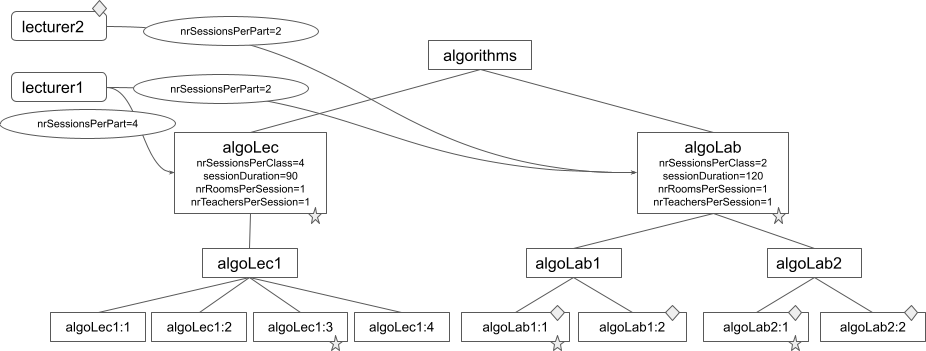
\includegraphics[scale=0.35]{img/utp_rule_1.png}


\newcounter{save_equation}
\setcounter{save_equation}{\value{equation}}
\setcounter{equation}{0}

\renewcommand{\theequation}{R\arabic{equation}}

{\footnotesize{
\begin{flalign}
&\texttt{{\FORBIDDENPERIOD}((<(\TEACHER,{lecturer2},\_)>,9120,9240)}
&\label{rule-example-1}
\\
&\texttt{{\SEQUENCED}(<(\CLASS,\_,\myset{3}),(\PART,{algoLec},\_)>,
<(\CLASS,\_,\myset{1}),(\PART,{algoLab},\_)>)}
&\label{rule-example-2}
\end{flalign}
}}


\setcounter{equation}{0}
\renewcommand{\theequation}{C\arabic{equation}}

%
{
\footnotesize
\begin{flalign}
\nonumber &\texttt{{\FORBIDDENPERIOD}((lecturer2,\{algoLab1:1,algoLab1:2,algoLab2:1,algoLab2:2\}),}\\
 & \texttt{9120,9240)}
&\label{constraint-example-1}
\\
&\texttt{{\SEQUENCED}((algoLec1,\{algoLec1:3\}), (algoLab1,\{algoLab1:1\}))}
&\label{constraint-example-2}
\\
&\texttt{{\SEQUENCED}((algoLec1,\{algoLec1:3\}), (algoLab2,\{algoLab2:1\})}
&\label{constraint-example-3}
\end{flalign}
}
%

\caption{Rules flattening and corresponding constraints on a toy example.}
\label{fig:utp-rule-1}

\setcounter{equation}{\value{save_equation}}
\end{figure}


Figure~\ref{fig:utp-rule-1} illustrates the rules flattening process on a toy example.
Course \texttt{algorithms} is split into a lecture part \texttt{algoLec} and a lab part \texttt{algoLab}.
The lecture part has a single class of 4 sessions taught by \texttt{lecturer1} and the lab part has 2 classes of 2 sessions each taught by \texttt{lecturer1} or \texttt{lecturer2}.
%Figure~\ref{fig:utp-rule-1} illustrates the flattening of the following rules: 
%on a simple model consisting of 2 teachers and & course subdivided into 2 parts, 3 classes and 8 sessions. The first rule forbids a time period for 
Rule~\ref{rule-example-1} %below
requires that \texttt{lecturer2} has no session between slots $9120$ and $9240$, corresponding for instance to 8am and 10am on Tuesday of week 2. % assuming a granularity of 1 minute per time slot. 
%In this rule, $9120$ (resp. $9240$) is the value\footnote{Each possible session schedule is mapped to a single value. All possible values make up the domain of a session.} that corresponds to 8am on Tuesday (resp. 10am on Tuesday) of week 2. 
The selector includes no mask and no filter hence matches with all possible sessions of \texttt{lecturer2} 
as indicated with diamonds on Figure~\ref{fig:utp-rule-1}. 
The resulting domain of e-maps is the singleton $\myset{(lecturer2,\map{\TEACHER}{\SESSION}{lecturer2})}$
and the rule is flattened into a single \texttt{\FORBIDDENPERIOD} constraint (\ref{constraint-example-1}). %$\myset{\map{\TEACHER}{\SESSION}{teacher2}}$.
Rule~\ref{rule-example-2}
%requires that the first practical session in Algorithmic \todo[inline]{Marc : pourquoi algo ?} start after the third lecture.
requires that the first sessions of the labs start after the third lecture.
The two selectors include a filter. The first selector matches with all class sessions of rank 3 in part \texttt{algoLec}, 
and the second matches with all class sessions of rank 1 in part \texttt{algoLab} as indicated with stars on the figure.
The rule is flattened into 2 \texttt{\SEQUENCED} constraints (\ref{constraint-example-2} and \ref{constraint-example-3}) corresponding to the cross product of the e-map domains 
%$\myset{(algoLec1,\map{\RANK}{\SESSION}{3}\cap\map{\PART}{\SESSION}{algoLec})}$
%and $\myset{(algoPra1,\map{\RANK}{\SESSION}{1}\cap\map{\PART}{\SESSION}{algoPra}),(algoPra2,\map{\RANK}{\SESSION}{1}\cap\map{\PART}{\SESSION}{algoPra})}$.
$\myset{(algoLec1,\myset{s\in\SESSION\ |\ \sessionrank{s}=3}\cap\map{\PART}{\SESSION}{algoLec})}$
and $\myset{(algoLab1,\myset{s\in\SESSION\ |\ \sessionrank{s}=1}\cap\map{\PART}{\SESSION}{algoLab}),(algoLab2,\myset{s\in\SESSION\ |\ \sessionrank{s}=1}\cap\map{\PART}{\SESSION}{algoLab})}$.
\coco{Core constraint }

% \input{2-1-1-variables-table}
% \input{2-1-1-core-constraints-table}
% The constraint~\ref{ctr:allowedslots} restricts the set of possible values to the allocated starting slots in the corresponding course part for a session. Similarly, constraint~\ref{ctr:allowedrooms} limits the set of possible values to the allocated rooms in the corresponding course part for a session. Likewise, for teachers, constraint~\ref{ctr:allowedteachers} restricts the set of possible teachers.

% To express the desired number of rooms per course session, we refer to cardinality constraint~\ref{ctr:cardinalmultiroom}, while for teachers, we reference constraint~\ref{ctr:cardinalmultiteacher}. Constraint~\ref{ctr:cumulativeroomcapacity} specifies that each session must take place in a set of rooms whose cumulative capacity can accommodate the groups enrollment of the session.

% More generally, constraint~\ref{ctr:roomuse} prohibits the cumulative capacity of sessions taking place in a room, for a given time slot, don't exceeding the room's capacity. Constraint~\ref{ctr:nooverlap2days} ensures that no session spans across two different days. 
% %Note that sessions are considered uninterruptible and, in particular, may not overlap two days. 
% Finally, constraint~\ref{ctr:coresumvariables} establishes the relationship between auxiliary time values and the starting slot variable for each session.

% For each teacher is allocated a fixed number of sessions in each course part he is eligible for, leaving lecturer-to-session assignment decisions to solvers (\hyperref[feat:service]{``service''}) and we used the constraint required\_teacher to explain this relation. And symmetrically, each room allowed to %
% %in a course part may be freely allocated to any session of the part (possibly none \hyperref[feat:roommodal]{``no room''}) but 
% the model provides the flexibility to mark a room as mandatory (e.g., requiredRooms constraint) in which case it will host or co-host all the sessions\hyperref[feat:ressourcedistribution]{``ressource distribution''}. 


